\chapter{Introduction}




\section{Diffraction and the SEM}


The Venn diagram of electron diffraction and scanning electron microscopy (SEM), shown here in Fig.~\ref{Fig:Venn}, is showing a very small overlap. Diffraction in general, and particularly that of electrons, which  we will discuss in more details in Chapter~\ref{Chap:Diffraction} from page~\pageref{Chap:Diffraction}, is a mature and well understood subject. So is the now ubiquitous materials investigation tool that is the SEM, which we will briefly cover on page~\pageref{sec:sem}. 

\begin{figure}[ht]
\centering
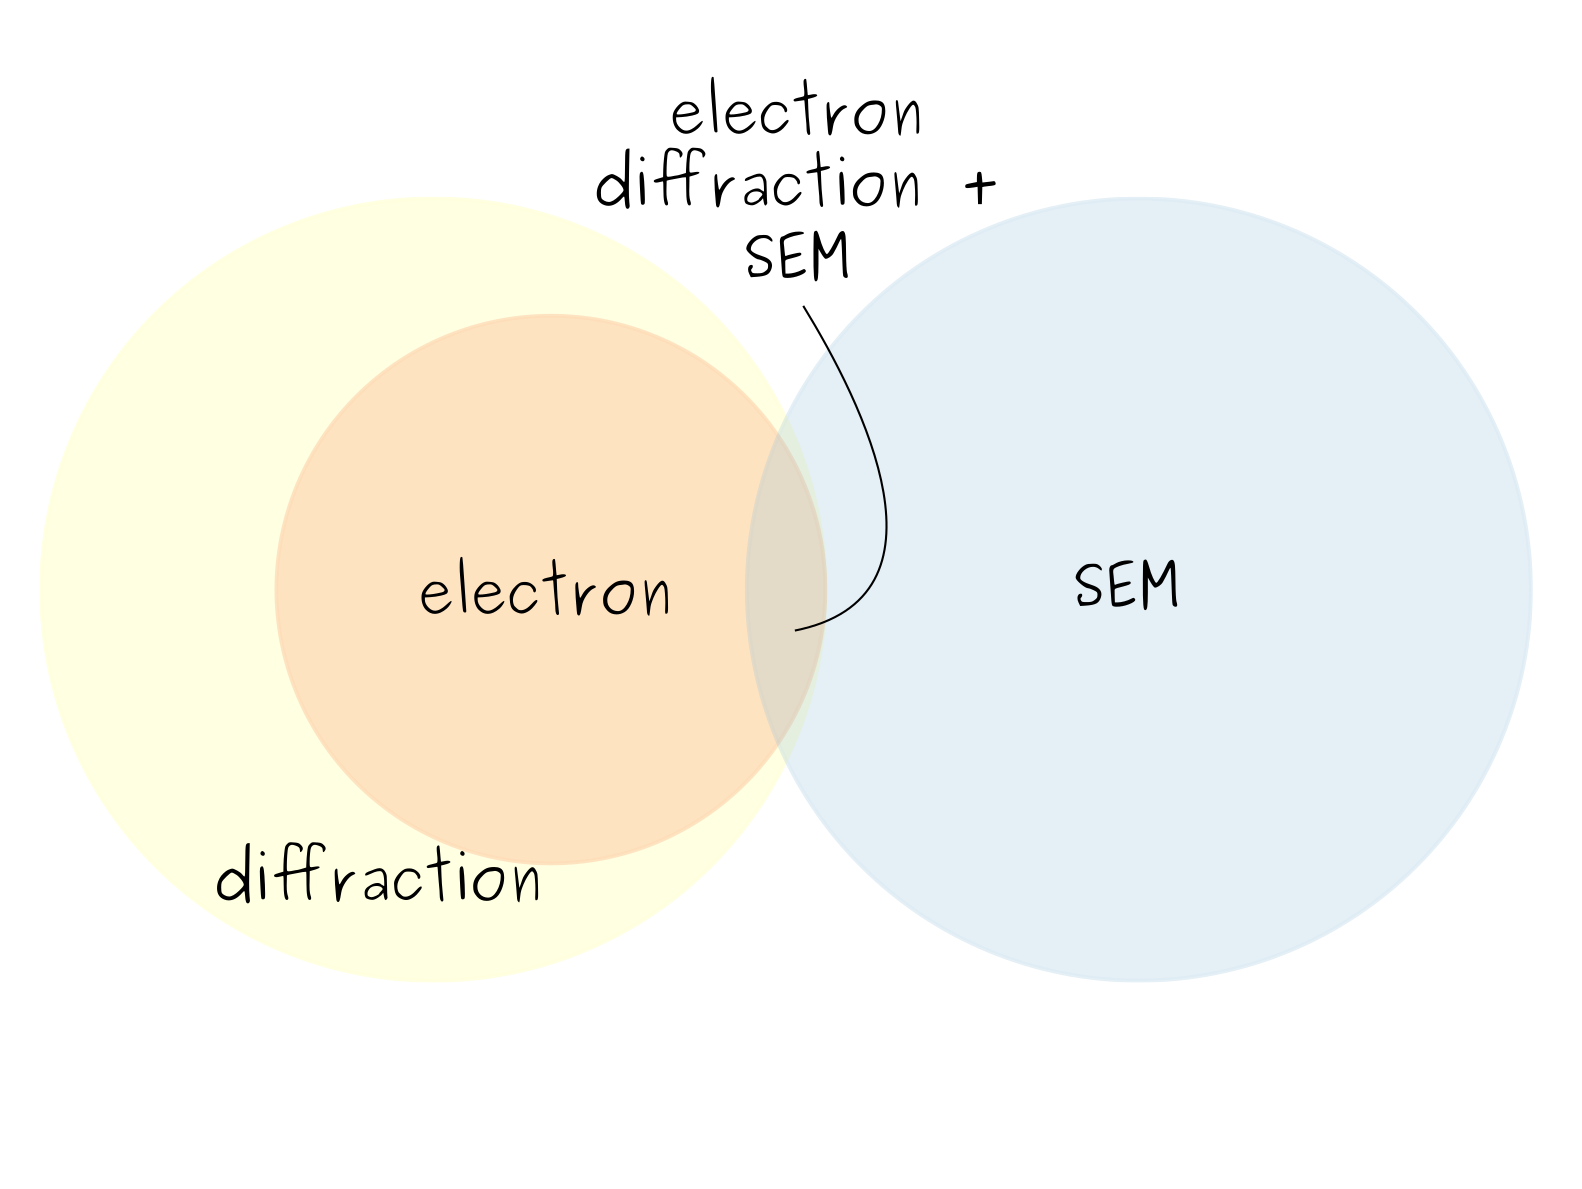
\includegraphics[width=0.71\linewidth]{Figures/VenSEM.png}
\caption[SEM and electron diffraction Venn diagram.]{Venn diagram showing how many Google scholar results contain the keywords: diffraction (yellow), electron diffraction (orange) and SEM (blue). The small overlap  summarises the topics addressed in this Thesis. The area of the circles is proportional to the number of search results.}
\label{Fig:Venn}
\end{figure}

The group of people engaged in studying both these fields is a very select one. The techniques based on electrons diffraction in the SEM either do not have a dedicated conference such as the \textit{channelling} family; this includes electron channelling patterns (ECPs) and electron channelling contrast imaging (ECCI) -- which we will explore in Chapter~\ref{chap:ECCI} from page~\pageref{chap:ECCI}--, or do have dedicated conferences; this is the case for the backscattered/fore-scattered diffraction family which includes electron backscattered diffraction (EBSD) and, more recently, transmission Kikuchi diffraction (TKD), which will be described in Chapter~\ref{chap:TKD} from page~\pageref{chap:TKD}, but are dominated by material scientists interested more in understanding the materials rather than the physics of the characterisation technique. 



Some of these techniques are more novel than the others, but all of them carry mysteries about aspects of the underlying physical processes. These unanswered questions are enticing not only from the aspect of fundamental physics, but also as a promise of more information that could be derived from these measurements. Building and implementing models that accurately predict these behaviours is, therefore, an important aspect of the field. 

In Chapter~\ref{chap:ECCI} I talk about ECCI, a SEM diffraction method  well suited for the characterisation of threading dislocations (TDs) in nitrates. Then, in Chapter~\ref{chap:TKD} I talk about TKD, a SEM diffraction technique optimised for the study of truly nano-crystalline materials.  





\subsection{Diffraction}

Starting with page~\pageref{Chap:Diffraction}, I will spend the entire chapter~\ref{Chap:Diffraction} on the powerful characterisation technique that is diffraction. There are only handful more elegant ideas out there than the power of observing the reciprocal space of an ordered arrangement of atoms, taking us very quickly to the conundrum of why is maths such a good description of reality.  But let us not digress. 

The geometry of diffraction is beautifully simple in the form of Bragg's law. Perhaps less intuitive is the fact that Braggs law being satisfied is not a guarantee of non-zero diffracted intensity. This behaviour is going to depend not only on the crystal system as Bragg law does, but instead it is going to be a map of the space group symmetry of the material under investigation. 

It is important to understand the basic diffraction behaviour in a material system before trying to derive information from a diffraction based technique applied to that material system. I will show, in Chapter~\ref{Chap:Diffraction}, theoretical predictions for electron diffraction relating parameters, such as scattering and structure factor, for a few group-III nitride materials: AlN, GaN and InN. 

While all particles diffract in the same way, electrons interact more strongly with matter and simplifications that can be done in the more established case of X-ray diffraction predictions are not acceptable when it comes to electrons. In the rest of that Chapter~\ref{Chap:Diffraction} I will review the dynamical model of electron diffraction and show how it incorporates the diffraction parameters mentioned above.

Because we cannot talk about diffraction without some solid knowledge of crystallography, I cover extensively the basics of crystallography and crystallographic computations in Chapter~\ref{chap:Background}. Since diffraction is the map of the crystal symmetry I examine in Appendix~\ref{Chap:Symmetry} on page~\pageref{Chap:Symmetry} the full $\mathbf{P6_3mc}$ symmetry of the wurtzite system.  

\subsection{The scanning electron microscope}
\label{sec:sem}
% microscopy
The phenomena described in the previous section occur at a scale too small to be measured by the naked eye. Luckily,  development of science had brought us two main extensions  to the range of scales we can study. On one hand,  the telescope brings very distant objects closer and is optimised to collect as much light as possible and, on the other, the microscope makes very close objects appear many times larger.
Interestingly, both these aids can be traced back to a \nth{17} century event: the development of glass lenses used in spectacles. Fundamentally, both these visual extensions are governed by the same optics laws. 

While modern light microscopes can commonly\footnote{ Developments in super resolution optical microscopy show that certain applications can overcome Abbe's limit.} showcase a magnification of about $2000\times$, their spatial resolution is limited by the wavelength of visible light, which is of the order of hundreds of nanometers, through Abbe's equation. One way around it is to use  different imaging particles, for instance, X-rays or electrons which have significantly smaller wavelengths (see Table~\ref{table:diffractingParticles} for wavelength comparison between X-ray photons and electrons).   

We will explore further the electron microscope, excellent detailed descriptions of which can be found in ref.~\cite{Hearle72} and ref.~\cite{reimerSEM}. There are various ways of generating an electron beam. For instance, in our (FEI now Thermo Fisher) SEM, a field enhanced thermionic emission Schottky gun is used to generate a beam of electrons. This beam is then focused through a series of condenser lenses onto the surface of a sample such that the beam spot size on the sample can go down to  \SI{1}{\nano \meter} in diameter in practice.  After the beam is focused on the sample, scanning coils are used to deflect the beam on a set of orthogonal directions in a predefined manner. 

Depending on the geometry of imaging\footnote{ But also electron beam energy and sample preparation procedure.} we can loosely classify electron microscopy into \textit{transmission electron microscopy} (TEM) on one hand, where the image is formed by electrons which have travelled through a very thin sample, and \textit{scanning electron microscopy} (SEM), where the imaging electrons come from the same, top surface of the sample with which the incident beam interacts\footnote{ Advances in both worlds make this distinction imperfect. There is an exception to the rule above, in the form of transmission SEM. To make things even harder to classify there is also scanning TEM.}. Both of them have advantages and disadvantages. The TEM geometry minimises the lateral spread of the electron-sample interaction volume providing therefore higher spatial resolution, but it also limits its field of view. Additionally, thinning the sample to the sizes required by this geometry can be cumbersome, time consuming and irremediably damaging to the sample. There is also the additional question the microscopist must answer, whether the features observed are intrinsic to the sample or were introduced during the polishing process. On the other hand, for non-biological materials, the SEM requires minimal sample preparation since the thickness of the sample does not limit its capabilities. The downside, as we will see, is that the SEM is not optimised for diffraction contrast in the same way the TEM is. 


Since electrons interact strongly with matter they can generate a plethora of signals for one to measure in the SEM using the right, specialised detector:
\begin{itemize}
    \item Most commonly, low-energy ($<$\SI{50}{\electronvolt}) \textit{secondary} electrons (SE) are ejected by those atoms with which the primary beam electrons have inelastically scattered. With such low energies these electron cannot come from very deep in the sample, which means the interaction volume is narrow enough to provide a tool for high resolution surface imaging. These electrons are collected by attracting them to an electrically biased grid and then further accelerated towards a phosphor screen or scintillator, in what is know as a Everhart-Thornley detector~\cite{ETdetector}.
    
    
    
    \item In addition to secondary electrons, excited atoms will also emit a variety of electromagnetic radiation such as characteristic X-rays which can provide information on the distribution of different elements in the sample as long as the SEM is equipped with wavelength dispersive \textit{X-ray spectrometers} (WDS) or energy-dispersive X-ray spectroscopy (EDS). 
    
    \item As the atoms relax back to their ground state after the encounter with the high energy electrons, they can generate light which can provide useful optical information in a technique known as \textit{cathodoluminescence} (CL)~\cite{Paul11}.
    
    \item The primary beam electrons will also escape the sample, after having a range of energies through inelastic scattering. This implies, that, at some point in their trajectory, the incident electrons suffered a large angle elastic scattering event such that they turn back to the surface of entry. All the incident electrons that suffer an elastic scattering event and manage to escape through the entry surface are collectively known as \textit{backscattered electrons} (BSE) and can be detected by a scintillator or a solid state detector. Since heavier atoms will elastically scatter electrons more strongly, BSEs can be used to detect contrast due different chemical compositions. Additionally, if the detector is not collecting a symmetric radial distribution of BSEs, then the image will also contain strong topographic contrast (for instance, think shadowing). 
    
 \begin{figure}[ht]
\centering
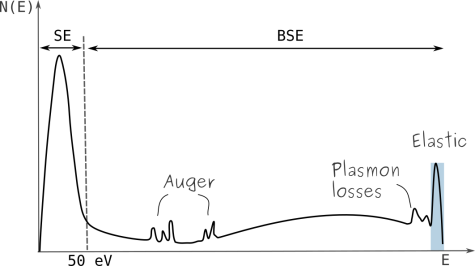
\includegraphics[width=0.62\linewidth]{Figures/spectrum.png}
\caption[SEM electrons energy spectrum.]{Schematic energy spectrum of secondary and backscattered electrons in an SEM [after~\cite{bell12}].}
\label{Fig:Espectrum}
\end{figure}

    \item Figure~\ref{Fig:Espectrum} shows the energy distribution of electrons reaching the BSE detector for an incident beam of energy $E$. Superimposed on the BSE energy curve are a few other signals but we will only talk here about the elastic peak as it it at the core of this work. A subset of BSEs will lose almost no energy before reaching the detector, either because they have been backscattered by the top layer of the sample, or, more likely, because they underwent diffraction, a case in which inelastic scattering processes are reduced (see the discussion on channelling on page~\pageref{sec:channelling}). We will call these the \textit{elastically BSEs}. This signal can provide information on the crystallographic orientation of a small region of the sample or about small changes in local strain. More on this in Chapter~\ref{chap:ECCI} and Chapter~\ref{chap:TKD}. One could use energy sensitive detectors to select only this signal~\cite{Stefano}.
\end{itemize}




We will be concerned in this Thesis only with elastically scattered BSEs (in Chapter~\ref{chap:TKD} we will also talk about forward scattered electrons (FSE)). The sample geometry optimised for this signal is shown below in Fig.~\ref{Fig:sillySEM}. The sample is tilted with respect to the incident beam and the detector is positioned such that it can collect the solid angle of the backscattered electrons that provides the highest intensity. We call this geometry forward-scattering. 



\vspace{0.2cm}

\noindent\begin{minipage}{0.5\textwidth}
The method of operation of the SEM is shown Figure~\ref{Fig:sillySEM}. A collimated beam of electrons is focused on the surface of a tilted sample. The beam is then scanned in a raster manner over the area of interest on the sample. The detector collects one pixel worth of BSEs intensity at a time. The beam is moved by the deflector coil to the next position on the sample defined by the step size. The resulting image is made up of the ordered collected pixels, and, at the end of the scan, has as many pixels as steps used in scanning.  
\end{minipage}%
\begin{minipage}{0.5\textwidth}
    \centering
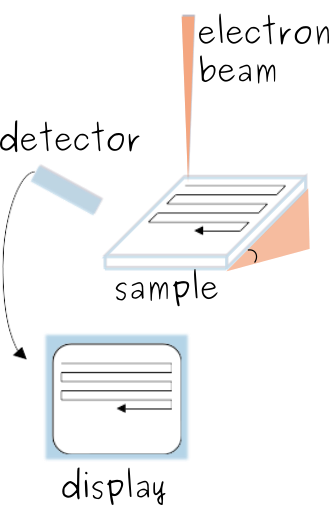
\includegraphics[width=0.48\linewidth]{Figures/sillySEM.png}
\captionsetup{width=.7\linewidth}
\captionof{figure}{SEM schematics in forward-scattering geometry.}
\label{Fig:sillySEM}
\end{minipage}

\vspace{0.4cm}



% TILT
The tilt of the sample in the forward-scattered geometry in the SEM ensures that  enough electrons reach the detector. It also makes the geometry of diffraction very different from that in the TEM. The sample's z-direction in the SEM is not the same as the beam direction which is the case for the TEM sample geometry. This means that if we are to use the diffraction models developed for TEM, they must be generalised for the sample tilt.  More about this in the next chapter. 

References~\cite{Hearle72, reimerSEM} discuss the electron optics and we will not delve  into here. We will however mention that the tilt of the sample affects the ``squareness'' of the scanned area. The trapezoidal area being scanned will produce a distorted image, which can be corrected to some degree using the tilt correction function (see page 50 in ref.~\cite{SEMbooklet} for tilt correction artefacts). The tilt can also change the shape of the beam on the sample which not only affects the imaging but also the diffraction interaction volume. 


%relativistic correction
Let us briefly address relativistic corrections and the correction factor, $\gamma$,  for electrons used in electron microscopy. The de Broglie equation for the relativistic electron  wavelength, $\lambda$, can be approximated in terms of the accelerating voltage $V$ (equation 2.4 in \cite{goodhew88}) as:
\begin{equation}
    \lambda \approx \sqrt{\frac{150}{V + 10^{-6}\, V^2}}
\end{equation}
where the second term in the denominator  is due to Lorentz factor and only becomes important for voltages greater than $20$ \si{\kilo \electronvolt} as we can see in Table~\ref{Table:wavelength}. For SEM applications discussed in this work we will focus on $20$ \si{\kilo \electronvolt} incident electrons, and discard, quite acceptably, relativistic effects. 

\begin{table}[ht]
\caption{Corrected and uncorrected electron wavelengths for voltages used in  electron microscopy.}
\label{Table:wavelength}
\vspace{-0.4cm}
\centering
\begin{longtable}{l c c c}\toprule
             \multirow{2}{*}{\tabhead{Voltage [\si{\kilo \electronvolt}] }} &  \multirow{2}{*}{\tabhead{Lorentz factor $\gamma$} \hspace{0.4cm}}  & \multicolumn{2}{c}{\tabhead{Wavelength  $\lambda$ [\si{\angstrom}]}}\\ \cmidrule{3-4}
              &  &\tabhead{Uncorrected}        &  \tabhead{Corrected}  \\ \midrule
20   & 1.04  & 0.086 & 0.086  \\
100  & 1.20  & 0.039 & 0.037  \\
1000 & 2.93  & 0.012 & 0.009  \\
\bottomrule
\end{longtable}
\end{table}


%%
\section{ECCI and the characterisation of TDs in nitrides  }
\label{sec:ECCITDmotivation}

Over the past thirty years there has been no shortage of interest in electronic and light emitting devices based on semiconductors and, as a result, their impact on modern technologies has become notable. Brighter, more efficient and more reliable light sources have been developed. Specifically, the group III-nitride material systems and their alloys have been intensely studied due to a number of promising properties. We have witnessed an ever increasing  span of emerging applications: from ultraviolet light water purification and hydrogen production, to high power electronics and novel optical communication systems~\cite{Kneissl10}. The bottleneck of developing the next generation devices remains the material science of improving even further the efficiency for these devices.

 The large difference in covalent bondings of the elements in these systems translates to greatly varying physical properties, including different lattice parameters and energy band gaps. The latter means that nitride alloy systems can offer a wide range of direct energy-band gaps, \ie high intensity luminescence at a wide range of wavelengths (\eg the band gap of InAlGaN systems ranges from infra-red to the ultraviolet region).  In addition, their structural stability at high temperatures and good thermal conductivity make them ideal candidates for the fabrication of high power transistors. GaN is a binary system belonging to this material group and together with its cousins, InN and AlN, and their ternary and quaternary alloys are one of the semiconductors on top\footnote{After the big ones like Si and Ge and the more established systems of arsenides and phosphides} of material scientists minds, due to their many applications in optical and electrical devices.  

Nevertheless, unlike Si and Ge, the group III-nitrides epitaxial growth is challenging due to the lack of a suitably lattice matched material. The lattice mismatch can be significant and the usual compromise between cost and growth impairment is sapphire ($Al_2O_3$), which at room temperature and along the $r$-plane has a lattice mismatch of $\sim1.1\%$ even on a coincident lattice~\cite{nitrides} with GaN grown in the \hkl[0001] direction. The epitaxial layers will be further strained during the cooling down stage, such that, at the end of the growth process, a thick layer can relax through the formation of dislocations along the interface of lattice mismatched materials.

An interface misfit dislocation introduces a discontinuous strain in the crystalline lattice, and the way to resolve the discontinuity is through the generation of \textit{threading dislocations} (TDs) which run from the layer interface through the crystal up to its surface. Dislocations and line defects of crystalline solids can strongly affect the properties of the material and the performance of the devices we would like to use these materials for.

Surprisingly, the blue emitting devices based on III-nitrides are able to function even in the presence of TD  densities of the order of $10^{11}$cm$^{-2}$, due to carrier localisation effects~\cite{Graham}. However, for a great number of devices, TDs prove to be problematic as they tend to be associated with impaired optical and electrical performances. For example, TDs correlate with increased leakage currents in green and blue light emitting diodes (LEDs) \cite{Ferdous} and overall reduction in efficiency in near-UV LEDs~\cite{Kamiyama}. Moreover, TDs can be blamed for reducing the lifespan of laser diodes as well as decreasing the electron mobility in high electron mobility transistors~\cite{Bougrioua}. TDs can cause premature junction breakdowns as well as inhibiting high current gains in GaN based UV avalanche photodiodes~\cite{Limb}. They are also connected to the current collapse in GaN field-effect transistors~\cite{Disanto} and the general degradation in performance of high power GaN based devices. Therefore, the need to study the origin, development and impact of TDs becomes apparent if we are to optimise growth methods aimed at reducing the TDs density.



%-------
\begin{figure}
\centering
\noindent\begin{minipage}{0.47\textwidth}
    \centering
    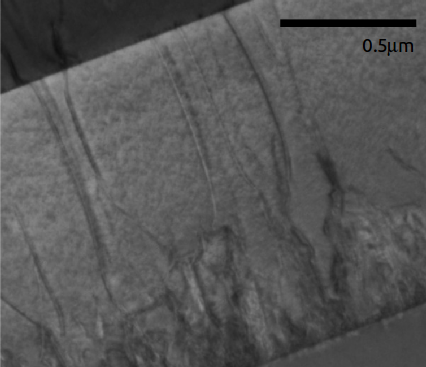
\includegraphics[width=0.9\linewidth, height=0.25\textheight]{Figures/TEM.png}
    \captionsetup{width=0.8\linewidth}
    \caption[AlGaN TEM.]{Transversal TEM image\footnote{Taken at the Kelvin Nanocharacterisation Center, University of Glasgow. ~~By permission of David Thomson, University of Strathclyde} of an AlGaN on sapphire showing threading dislocations reaching an interface.}
     \label{fig:tem}
\end{minipage}
\;\;\;
\begin{minipage}{0.48\textwidth}
     \centering
     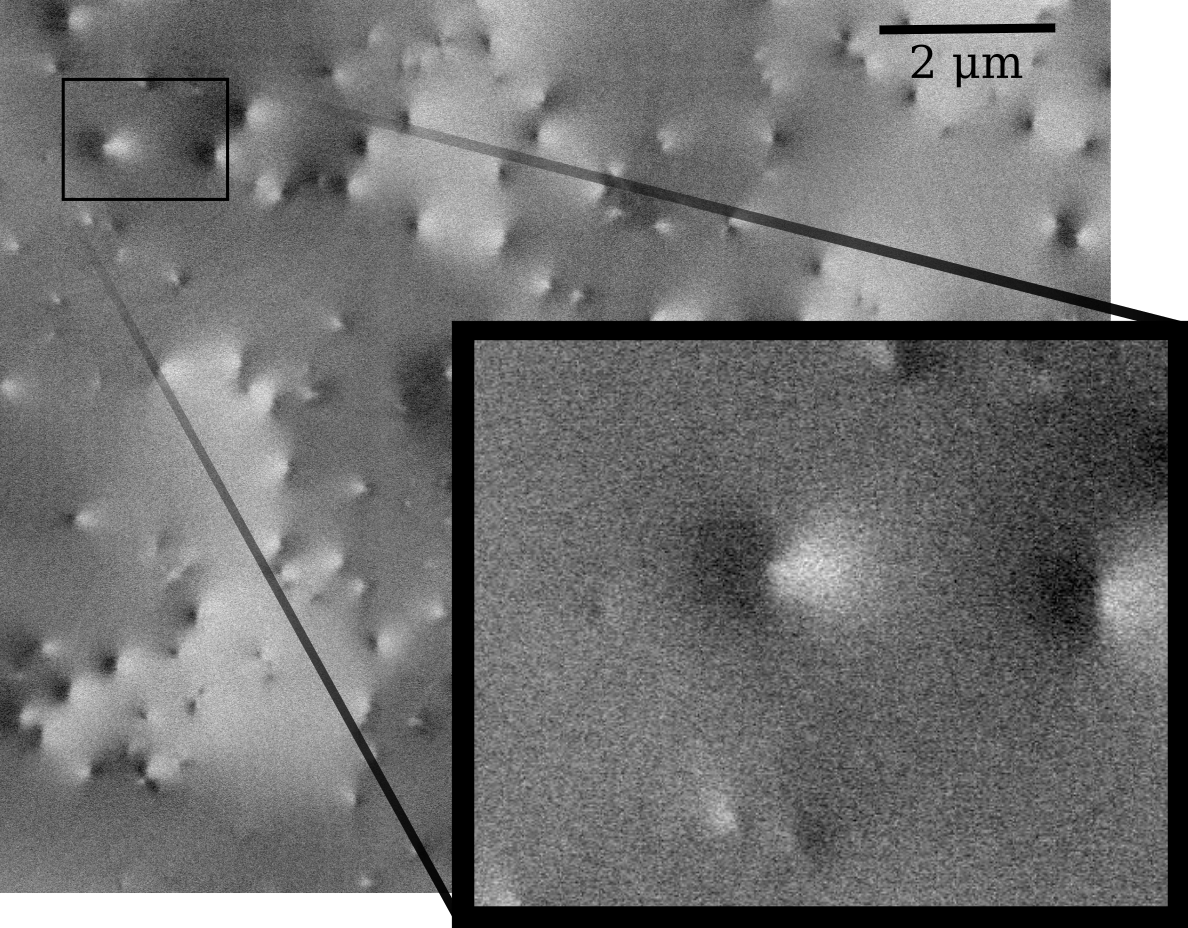
\includegraphics[width=0.9\linewidth, height=0.25\textheight]{Figures/ECCI.png}
      \captionsetup{width=0.8\linewidth}
     \caption[GaN ECCI.]{Plan view ECC image\footnote{By permission of Allehiani Nouf Mohammad, University of Strathclyde} of a \hkl[0001] GaN on sapphire showing black-white contrast around threading dislocations.}
     \label{fig:ecci}
\end{minipage}
\end{figure}
%---------

Electron diffraction is one mechanism that is sensitive to the presence of strain due to dislocations in the crystal, facilitating therefore dislocation imaging. Transmission electron microscopy (TEM) has established itself as the default technique for the study of lattice deformations and for identifying defect types. We will talk more about dislocations in the next section but for now it is useful to know that two extreme \hkl[0001] threading dislocation characters can be distinguished: pure screw type (or \textit{\textbf{c}-type}) where the Burgers vector (\textbf{b}) is aligned along the \textit{c}-axis and pure edge dislocation (or \textit{\textbf{a}-type}) when the Burgers vector is confined to the (0001) basal plane. If neither of these conditions is strictly met, the dislocation is called mixed, or \textit{\textbf{a+c} type}.



TEM is especially reliable as a dislocation characterisation method as it can unambiguously identify  the \textbf{c} and \textbf{a} components of a dislocation line running parallel to the imaged surface. This is achieved through the application of certain relationships between the diffraction vector $\vb{g}$, Burgers vector $\mathbf{b}$ and the direction of the dislocation line $\mathbf{u}_l$ ($\vb{g} \cdot \vb{b} = 0$ and $\vb{g} \cdot \vb{b} \times \vb{ u}_l = 0$), known as the \textit{invisibility criteria}, for which no contrast associated
with \textbf{c} or \textbf{a} components can be observed. This method has been applied broadly in the study and
characterisation of dislocations in cross sectional GaN samples (\eg~\cite{Hino00}). For TDs which penetrate the sample surface normally (or almost normally) high resolution TEM (HRTEM) can provide direct observation of the Burgers vector direction of \textbf{a} type TDs. However, as the images are usually acquired in plan view, the \textbf{c} components are invisible. The destructive TEM sample preparation and its limited field of view can also restrict the number of defects that can be observed and hence may impact the statistical limits on estimating defect densities, particularly for materials with lower numbers of dislocations.


There are characterisation methods which do not share TEM’s requirements for sample preparation. These include atomic force microscopy (AFM), which can offer information on TDs associated with surface pits~\cite{Craven02} (often after an etching or decoration treatment) or when terminating step edges. However, AFM can be sensitive to surface debris and may require extended periods of time to image even relatively small areas~\cite{Koinkar97}. Alternatively, for larger area measurements, X-ray diffraction (XRD)~\cite{Heinke00} or cathodoluminescence~\cite{Rosner97} can provide information on the global material defect densities but can have serious limitations in terms of resolving individual dislocations, especially XRD. 

An alternative to the above methods is the use of the electron  channelling contrast imaging (ECCI) technique which can be employed within generally available field emission scanning electron microscopes (FE-SEMs). This approach can image defects with resolution of a few nanometers with a micrometer scale field of view, and is neither destructive nor based on direct sample contact. However, in order to obtain the maximum amount of information from these images, a thorough understanding of the contrast mechanisms is required.

Trager-Cowan \etal\cite{Carol} showed that using ECCI in the characterisation of nitrides is an excellent idea. ECCI has been used in the forescatter geometry to reveal extended defects and
morphological features of GaN samples while also delivering information about crystallographic orientation~\cite{Picard}. The electron channelling contrast images obtained in the SEM can provide structural information on dislocations  interacting with the sample surface, particularly when obtained in highly diffracting channelling conditions~\cite{Naresh}. This information is shown in the form of variation in the electron backscattered contrast intensity around a dislocation -- or dark-bright signal contrast on the micrograph. Because it can resolve individual dislocations while imaging larger areas (e.g. Nouf-Allehiani et al.~\cite{Nouf} for material with TDs having a mean separation of $\approx$ 200 nm), ECCI is an ideal candidate for both precise and accurate number estimates for a wide range of TD densities (\SI{e6}{\centi \metre^{-2}} -- \SI{e10}{\centi \metre^{-2}} ).


\subsection{What is Chapter~\ref{chap:ECCI} about?}


In this work I continue on the path of analysing the ECCI as a TD characterisation technique. In Chapter~\ref{chap:ECCI} I look at the theoretical models that could be applied to predict the TD contrast in ECC images of \hkl[0001] grown GaN. It was clear that the contrast predictions methods used for TEM will be inappropriate when considering contrast in bulk samples. If a TD dislocation in a thin TEM sample will introduce two opposite, and cancelling in effect, surface relaxations on the top and bottom surface, a beam in ECCI will only image the top surface and therefore be far more sensitive to the top surface relaxation. An model for ECCI contrast should therefore take into account the surface relaxation, to begin with. The questions I followed were \textit{What can a suitable model predict about the behaviour of the TD contrast?} and \textit{What can we then learn from this predicted behaviour?}.

Since diffraction conditions in the SEM are more challenging to pinpoint then in the TEM, I wanted to remove this hard to determine variable from the predictions and look, qualitatively, at the behaviour of a property that causes the contrast in the first place: the strain flavoured parameter that quantifies the correction to the deviation parameter $\beta$ due to the dislocation. I give it the name of \textit{ECC-strain}. 

By looking at isosurfaces of this newly minted ECC-strain for different types of dislocations in different conditions, I can make a few observations regarding the effect of geometry, the effect of dislocation type and the effect of diffraction condition on the imaged contrast. This observation can then be turned into recipes for contrast optimisation on one hand and dislocation characterisation on the other.



\section{TKD and study of truly nanostructured materials}





%Kikuchi patterns
Kikuchi patterns are another representation of the diffracting behaviour of electrons in the form of a variation in the angular distribution of escaping electrons undergoing diffraction, as we will see on page~\pageref{sec:Kikuchi}. We have already established that real materials are not perfect crystals. Dislocations are not the only imperfections that can dictate the properties of a carefully engineered material. The material structure can show features sometimes even at the nano scale level, in the form of crystal grains with more or less different crystal orientations from their neighbouring grains -- what we call polycrystals. 

The investigation and characterisation of the micro structure of new materials is a core aspect of materials science in particular but also fundamental science in general. Kikuchi diffraction became a widespread SEM technique, in the form of electron backscattered diffraction (EBSD), able to provide quantitative microstructural information about most inorganic crystalline materials. The history of Kikuchi diffraction patterns is almost ninety years old as we have seen on page~\pageref{table:historyDiff}, and the most applied version of it is in the form of EBSD.


However, recently, stimulated by the increased attention to nanostructured materials, which promise new and enhanced properties when compared to their larger scale counterparts, the interest in improving the resolution of established characterisation techniques has also expanded. The use of forward-scattered electrons (FSEs) through a thin sample as diffraction signal collected from the bottom of the foil has been shown to improve the lateral spatial resolution to below $10$ nm~\cite{Keller12, Trimby12}; this technique is commonly known as transmission Kikuchi diffraction (TKD) or transmission EBSD (t-EBSD). 

\subsection{What is Chapter~\ref{chap:TKD} about?}

The work described in Chapter~\ref{chap:TKD} was the outcome of a collaboration with Prof. Marc De Graef's group from Carnegie Mellon University. The CMU group developed a vast, open-source software called EMsoft~\cite{EMsoft} aimed at modelling a variety of diffraction techniques in the SEM including EBSD. 

The aim of our particular project was to add a TKD modality implementation in EMsoft. Since EMsoft comes with energy filtering abilities we showed that it provides more accurate indexing of patterns than the commercially available software can achieve. But, more importantly, being an open software, it also give us large data-set of information from which we can learn about the physics of electron scattering.  

In the resulting published paper~\cite{PascalTKD}  we compare the energy distributions of the different diffraction modalities of the SEM: ECP, EBSD and TKD. While Kikuchi like lines in ECPs are the result of electrons with a energies very close to the incident energy diffracting, in EBSD the relatively large interaction volume causes a spread of electron energies which in turn contributes to a blurring of the lines. On the other hand, for TKD we can predict that, in a sense, the sample thickness acts as an energy filtering mechanism. For samples thinner than the EBSD interaction volume the model predicts an increase in resolution of the Kikuchi bands which is observed experimentally. 